\documentclass[12pt,twoside]{scrartcl}
\usepackage[a4paper,top=2cm,left=2cm,right=2cm,bottom=2cm,includefoot,includehead]{geometry}
\usepackage{graphicx}
\usepackage[numbers]{natbib} % Add this line for natbib package
\usepackage{fancyhdr}
\usepackage{hyperref}
\usepackage{amsmath}
\usepackage{circuitikz}
\graphicspath{ {figures/} }


\ctikzset{
    resistor = american,
    % inductor = american,
    voltage = raised ,
    voltage dir = old,
    quadpoles/transformer core/inner = 1, %Eliminates the horizontal bars on the transformer
    quadpoles/transformer core/width = 0.8, %Adjusts the width so that the transformers are closer
    diodes/scale = 0.6,
    capacitors/scale = 0.6,
    resistors/scale = 0.6,
    inductors/scale = 0.8,
    % bipoles/label_distance = 4pt,
    % switch/scale = 0.8,
    % bipoles/length = 1cm,
}

%% shifted open voltage 
\tikzset{open shifted/.style={
    open ,open voltage position=legacy, voltage shift=-0.9}
}

\pagestyle{fancy} % Set the page style to fancy
\fancyhf{} % Clear all header and footer fields

% Define the header and footer content for odd and even pages
\fancyhead[CE,CO]{School of Electrical Engineering} % Left header on even pages, right header on odd pages
% \fancyhead[RE,LO]{Right Header} % Right header on even pages, left header on odd pages
\fancyfoot[LE,RO]{\thepage} % Page number on left footer of even pages and right footer of odd pages
\fancyfoot[RE,LO]{ELEC3251} % Left footer on odd pages, right footer on even pages

\begin{document}
\pagenumbering{arabic}
\setcounter{page}{1}
\begin{titlepage}
    \begin{center}

        
\includegraphics[width=0.2\textwidth]{LOGO_Square.pdf}

        \vspace*{0.4cm}
        School of Electrical Engineering \\
        University of Newcastle
        
        \vspace{1cm}
        \huge
        \textbf{\textsf{ELEC3251 \\ Assignment 1}}

        \vspace{0.5cm}
        \large
        \textbf{\textsf{Practical and Theoretical Analysis of \\ Buck Converter and Flyback Converter}}

        \vspace{1.5cm}
        \normalsize
        \begin{tabular}{l|r}
            Liam Patey-Dennis & c3349900 \\
            Joshua Thomas & c3376353
        \end{tabular}
        \vfill    
    \end{center}
\end{titlepage}


\section{Buck Converter}
\subsection{Ideal Calculations}
The duty cycle required to achieve an output voltage of $V_{o} = 5$ V for an input supply voltage of $V_{d} = 12$ V can be determined using the DC transfer function of the Buck converter, see Equation \ref{equation:Buck_TF}. The resulting duty cycle required for the ideal circuit is $D \approx 41.67$\%.\par
\begin{equation}
\frac{V_o}{V_d} = D \label{equation:Buck_TF}
\end{equation}
The output voltage ripple ($\Delta V_o$) of an ideal Buck converter is given by Equation \ref{equation:Buck_ripple}. This equation can be rearranged, see Equation \ref{equation:Buck_cap}, to find the required capacitance for the low pass filter, provided that the duty cycle ($D$), filter inductance ($L$), and switching period ($T_{s}$) are known. For $T_{s} = 1/f_{s} = 10$ $\mu$s, $L = 1$ mH, $D = 41.67$\%, $\Delta V_{o} = 25$ mV, and $V_o = 5$ V, the required capacitance is $C = 1.458$ $\mu$F. \par
\begin{equation}
\frac{\Delta V_{o}}{V_{o}} = \frac{1}{8}\frac{T_{s}^{2}(1-D)}{LC} \label{equation:Buck_ripple}
\end{equation}
\begin{equation}
C = \frac{V_o}{\Delta V_{o}}\frac{T_{s}^{2}(1-D)}{8L} \label{equation:Buck_cap}
\end{equation}
The output power of the converter will be limited by the ratings of the components in the circuit. As the output voltage of the converter is required to remain constant at $5$ V, only the output current can be adjusted to suit the ratings of the components. The inductor selected for the circuit is the Murata \#1410516C, which has a maximum DC current of $1.6$ A \cite{RNX0}. A IRFZ24NPbF MOSFET has been selected for the switch, this component has a maximum DC current rating of $17$ A \cite{RNX1}. The selected diode is an SB120 which has a maximum DC current of $1.0$ A \cite{RNX2}. The inductor current will equal the output current, assuming the voltage across the capacitor remains constant. Therefore, the output current must be less than $1.6$ A, to avoid causing damage to the inductor. The diode will only conduct when the switch is off, therefore the DC current flowing through the diode is $I_{D} = (1-D)I_{o}$. For $I_{o} = 1.6$ A the diode current is $0.93$ A, which is less than the maximum rating of the device. Therefore, the load resistance must be selected such that $I_{o} \le 1.6$ A. Using Ohm’s law this inequality is equivalent to $R_{Load} \ge 3.125$ $\Omega$. The smallest resistor provided in the laboratory kit is $3.9$ $\Omega$ so this resistance will be used for the load.\par
\vspace{5mm}
\noindent The continuous conduction mode (CCM) and discontinuous conduction mode (DCM) boundary occurs when the current flowing through the inductor reaches $0$ A. For the ideal Buck converter this will occur for a DC output current ($I_{oB}$) which can be found using Equation \ref{equation:Buck_DCM}. For the designed converter the minimum DC output current is $I_{oB} = 14.6$ mA, which is equivalent to an output load of $342$ $\Omega$.
\begin{equation}
I_{oB} \approx \frac{T_{s}V_{o}}{2L}(1-D) \label{equation:Buck_DCM}
\end{equation}
\pagebreak
\subsection{Ideal Simulations}
Wolfram System Modeller (Wolfram) was used to simulate the performance of the designed converter. The model used for the simulations is shown in Figure \ref{fig:Buck_idealModel}. The output voltage of the ideal Buck converter is shown in Figure \ref{fig:Buck_idealVout}. The average output voltage, at steady state, is close to 5 V which lies close to the theoretically expected value of 5 V. The slight discrepancy between the simulated value and the expected value may be the result of truncating the duty cycle to 2 decimal places ($5/12 \approx 0.4167$). It may also be a result of the numerical methods used by the Wolfram software to simulate the system. An output voltage ripple of 6.7 mV is observed from the simulations and is shown in Figure \ref{fig:Buck_idealRipple}.\par
\vspace{5mm}
\noindent Figure \ref{fig:buck_DCM} (A) displays the inductor current for a load resistance of 342 $\Omega$. The current reaches a minimum value of $120 $ $\mu$A, which indicates that the converter is close to the CCM-DCM boundary. Figure \ref{fig:buck_DCM} (b) displays the current for a load resistance of 345 $\Omega$. Slight distortion is observed in the waveform near the zero crossing which indicates that the converter has entered DCM. This suggests that the CCM-DCM boundary lies in the range $342 \le R_{Load} \le 345$ $\Omega$ which agrees with the theoretically expected value of 342 $\Omega$. The boundary may not lie exactly at 342 $\Omega$ because of the assumption, made in Equation \ref{equation:Buck_DCM}, that the inductor current and the output current are equal. This assumption is not correct as a small amount of current also flows through the capacitor.

\begin{figure}[h]
    \centering
    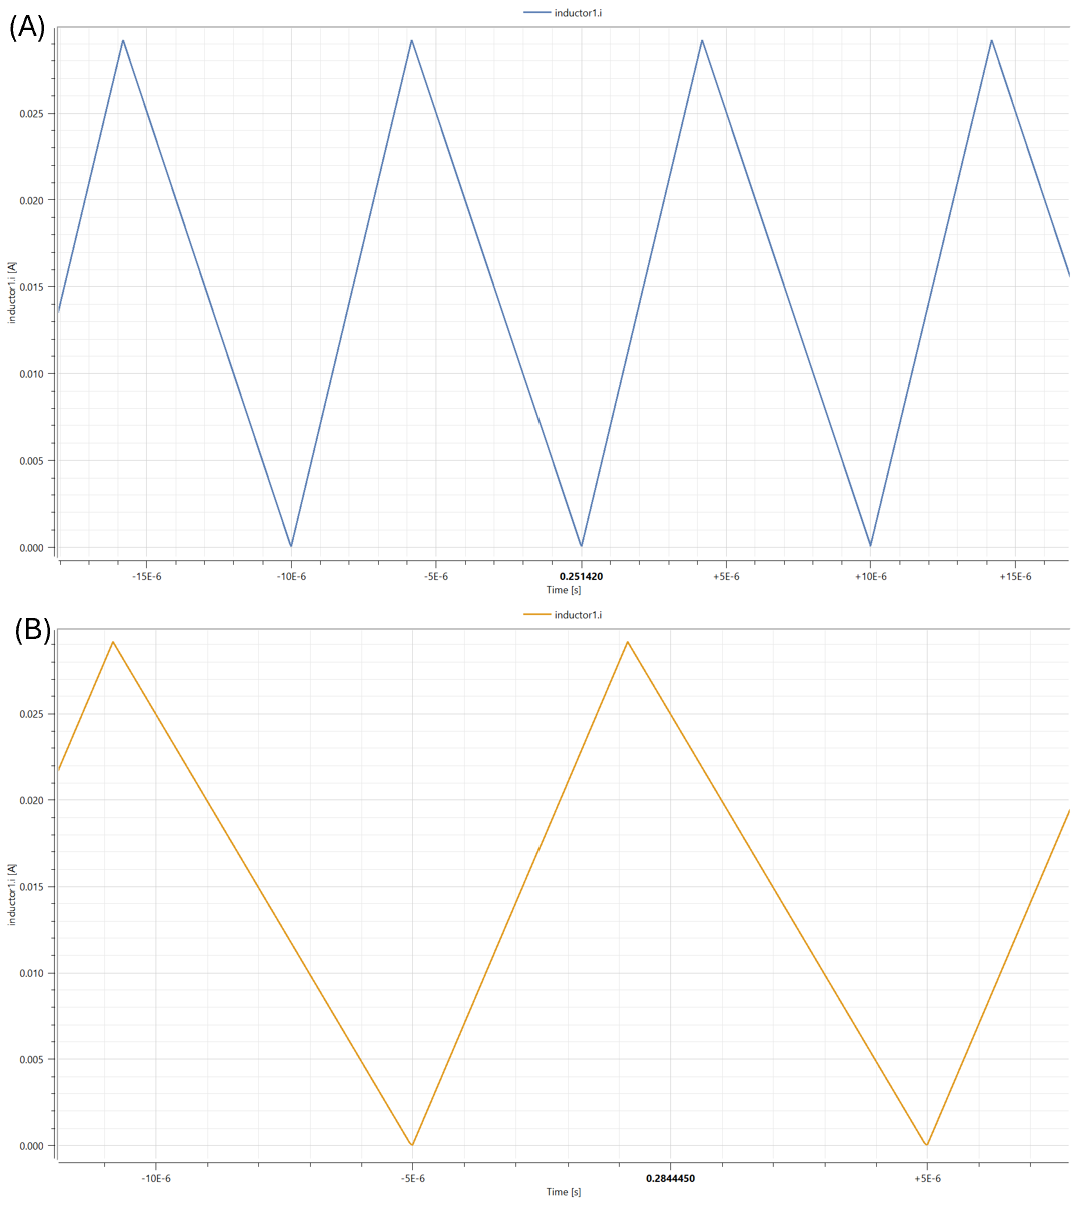
\includegraphics[width=0.6\textwidth]{buck_DCM}
    \caption{Buck converter inductor current for a load resistance of (A) 342 $\Omega$, and (B) 345 $\Omega$. A small amount of distortion is present in (B) which indicates that the CCM-DCM boundary lies in the range $342 \le R_{Load} \le 345$ $\Omega$.}
    \label{fig:buck_DCM}
\end{figure}
\newpage

\subsection{Non Ideal Calculations}
The previous calculations and simulations neglect many real-world effects that will affect the circuit's performance. Previously, no voltage losses were assumed to occur across the switch. This assumption is invalid as real switches are often implemented using transistors that have finite on resistances. Furthermore, it was assumed that no voltage drop occurs across the diode. All diodes have a non-zero voltage drop, which is required to overcome the potential barrier formed at the P-N junction of these devices. In addition, the windings of an inductor are not perfect conductors and hence have resistance. These effects will result in the output voltage of the converter being lower than the theoretically expected value. Figure \ref{fig:Buck_nonIdealCircuits} displays equivalent circuit models which can be used to account for these effects when (A) the switch is on and (B) when the switch is off. Applying Kirchoff’s voltage law (KVL) to the outer loop of each circuit, results in Equations \ref{equation:KVL_on} and \ref{equation:KVL_off}.
\begin{equation}
V_{L,on} = V_{d} - V_{o} - V_{loss, on} = V_{d} - V_{o} - (R_{DS}+ R_{L})i_{L} \label{equation:KVL_on}
\end{equation}
\begin{equation}
V_{L,off} = -V_{o} - V_{f} - V_{loss, off} = V_{o} - V_{f} - R_{L}i_{L}\label{equation:KVL_off}
\end{equation}
Where $R_{DS}$ is the on resistance of the switch, $R_{L}$ is the inductor resistance, and $V_{f}$ is the forward voltage of the diode.\par
\vspace{5mm}
\noindent If it is assumed that the circuit is in steady state, then the zero volt-seconds assumption can be applied which yields,
\begin{equation*}
V_{L,on}t_{on} + V_{L,off}t_{off} = 0
\end{equation*}
If the inductor current is assumed to be equal to the load current then,
\begin{equation*}
i_{L} \approx i_{Load} = \frac{V_{o}}{R_{Load}}
\end{equation*}
Which can be used with the previous equation to obtain Equation \ref{equation:Buck_nonIdealTF}.
\begin{align}
V_{o} &= \frac{R_{Load}}{(1+2D)R_{Load} - R_{L} - DR_{DS}}\left\{DV_{d} - (1-D)V_{f} \label{equation:Buck_nonIdealTF}\right\}
\end{align}
\noindent For the ideal duty cycle ($D = 41.67$\%) with the parameters $R_{DS} = 0.07$ $\Omega$, $R_{L} = 1.6$ $\Omega$, $V_{f} = 0.7$ V and a load current of $i_{L} = 1.28$ A ($R_{Load} = 3.9$ $\Omega$), the expected output voltage of the converter is $V_{o} =3.24$ V \cite{RNX1, RNX0, RNX2}. The duty cycle required to obtain an output of 5 V is $D = 61.44$\%.

INCLUDE EFFECTS OF INDUCTOR TOLERENCE AND LOAD TOLERENCE, MENTION PARASITICS

\newpage
\subsection{Non Ideal Simulations}
The output voltage of the non-ideal converter for the ideal duty cycle is shown in Figure \ref{fig:buck_NI_output_oldD}. Applying a 2nd order low pass filter, with a cutoff frequency of 10 kHz, to the output voltage results in average output voltage of 3.22 V which lies close to the theoretically predicted value of 3.24 V. Figure \ref{fig: buck_NI_output_newD} displays the output voltage for a duty cycle of 61.44 \%, an average voltage of 5.00 V is observed which matches the theoretically predicted value.

% \begin{figure}[h]
%     \centering
%     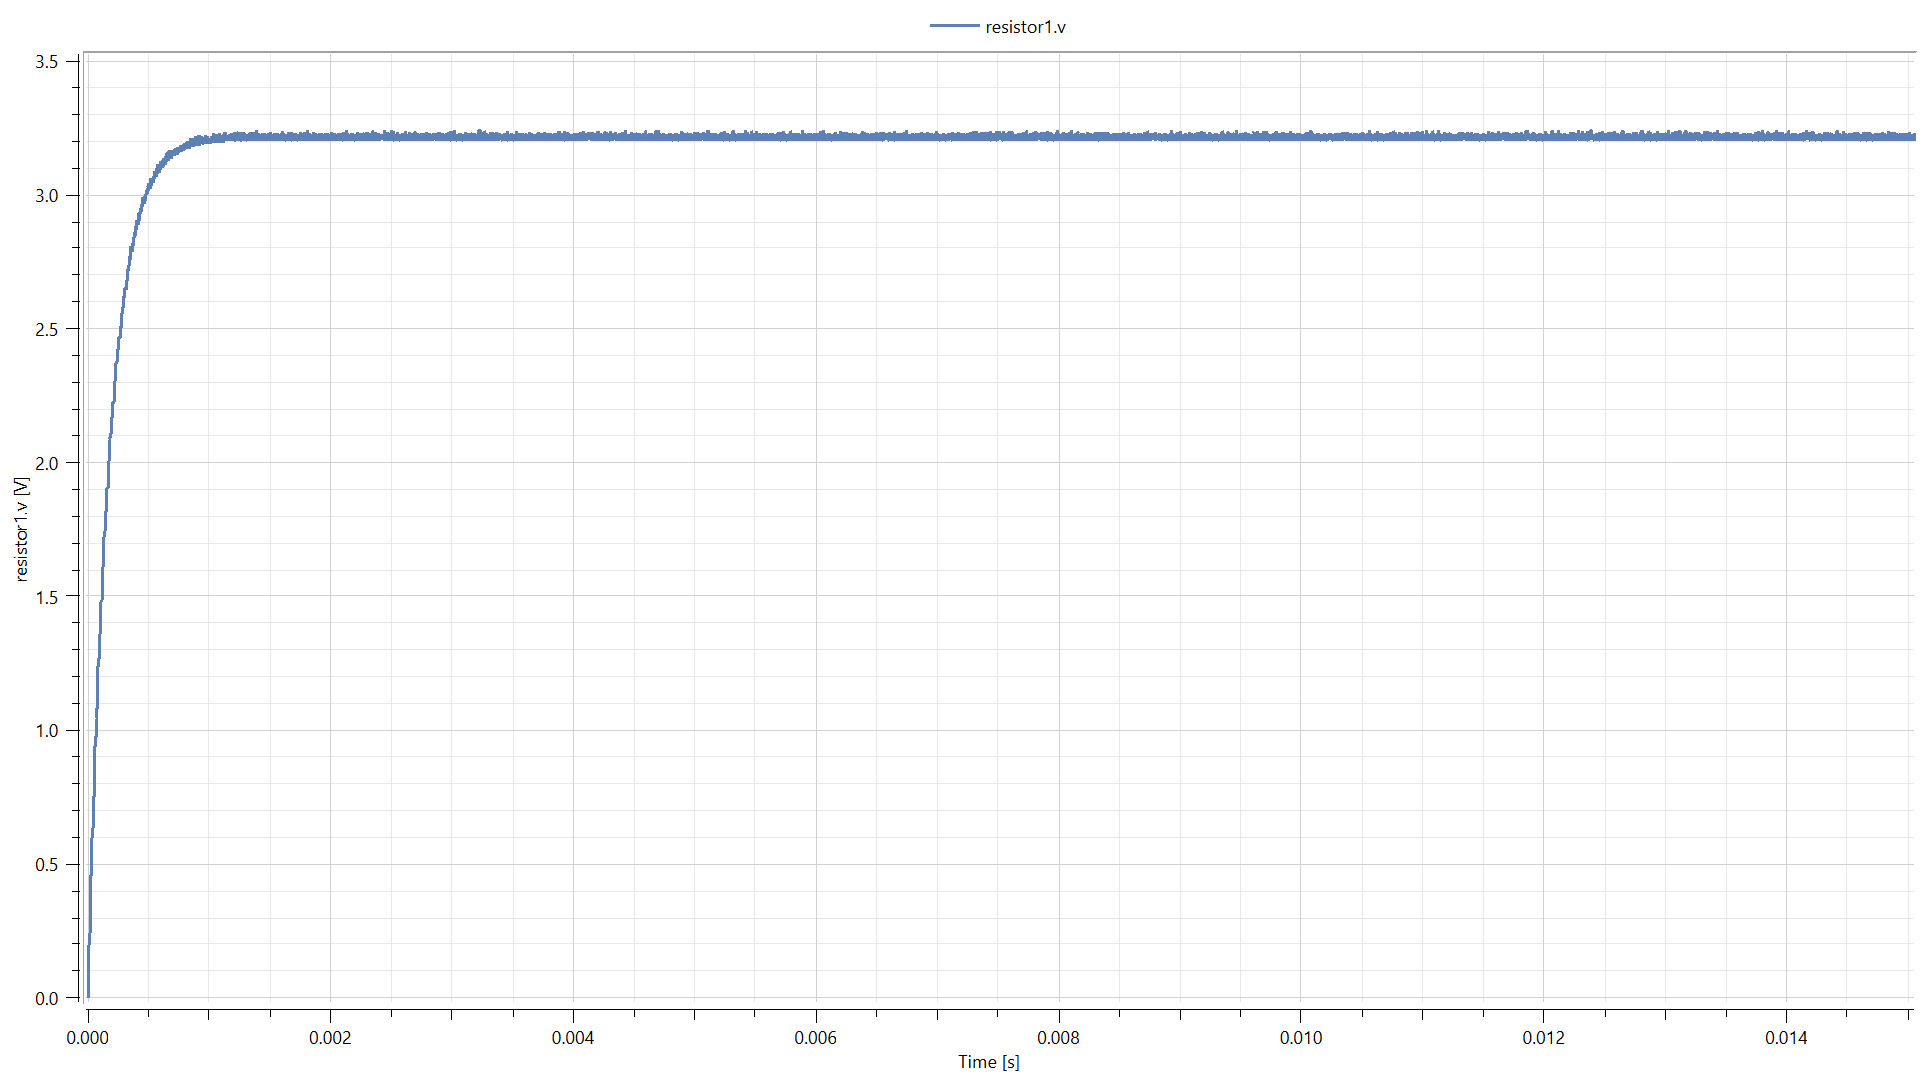
\includegraphics[width=0.6\textwidth]{buck_NI_output_oldD}
%     \caption{Non-ideal Buck converter output voltage for duty cycle of 41.67\% and a load of $3.9$ $\Omega$. An average voltage of 3.22 V is observed.}
%     \label{fig:buck_NI_output_oldD}
% \end{figure}
% \begin{figure}[h]
%     \centering
%     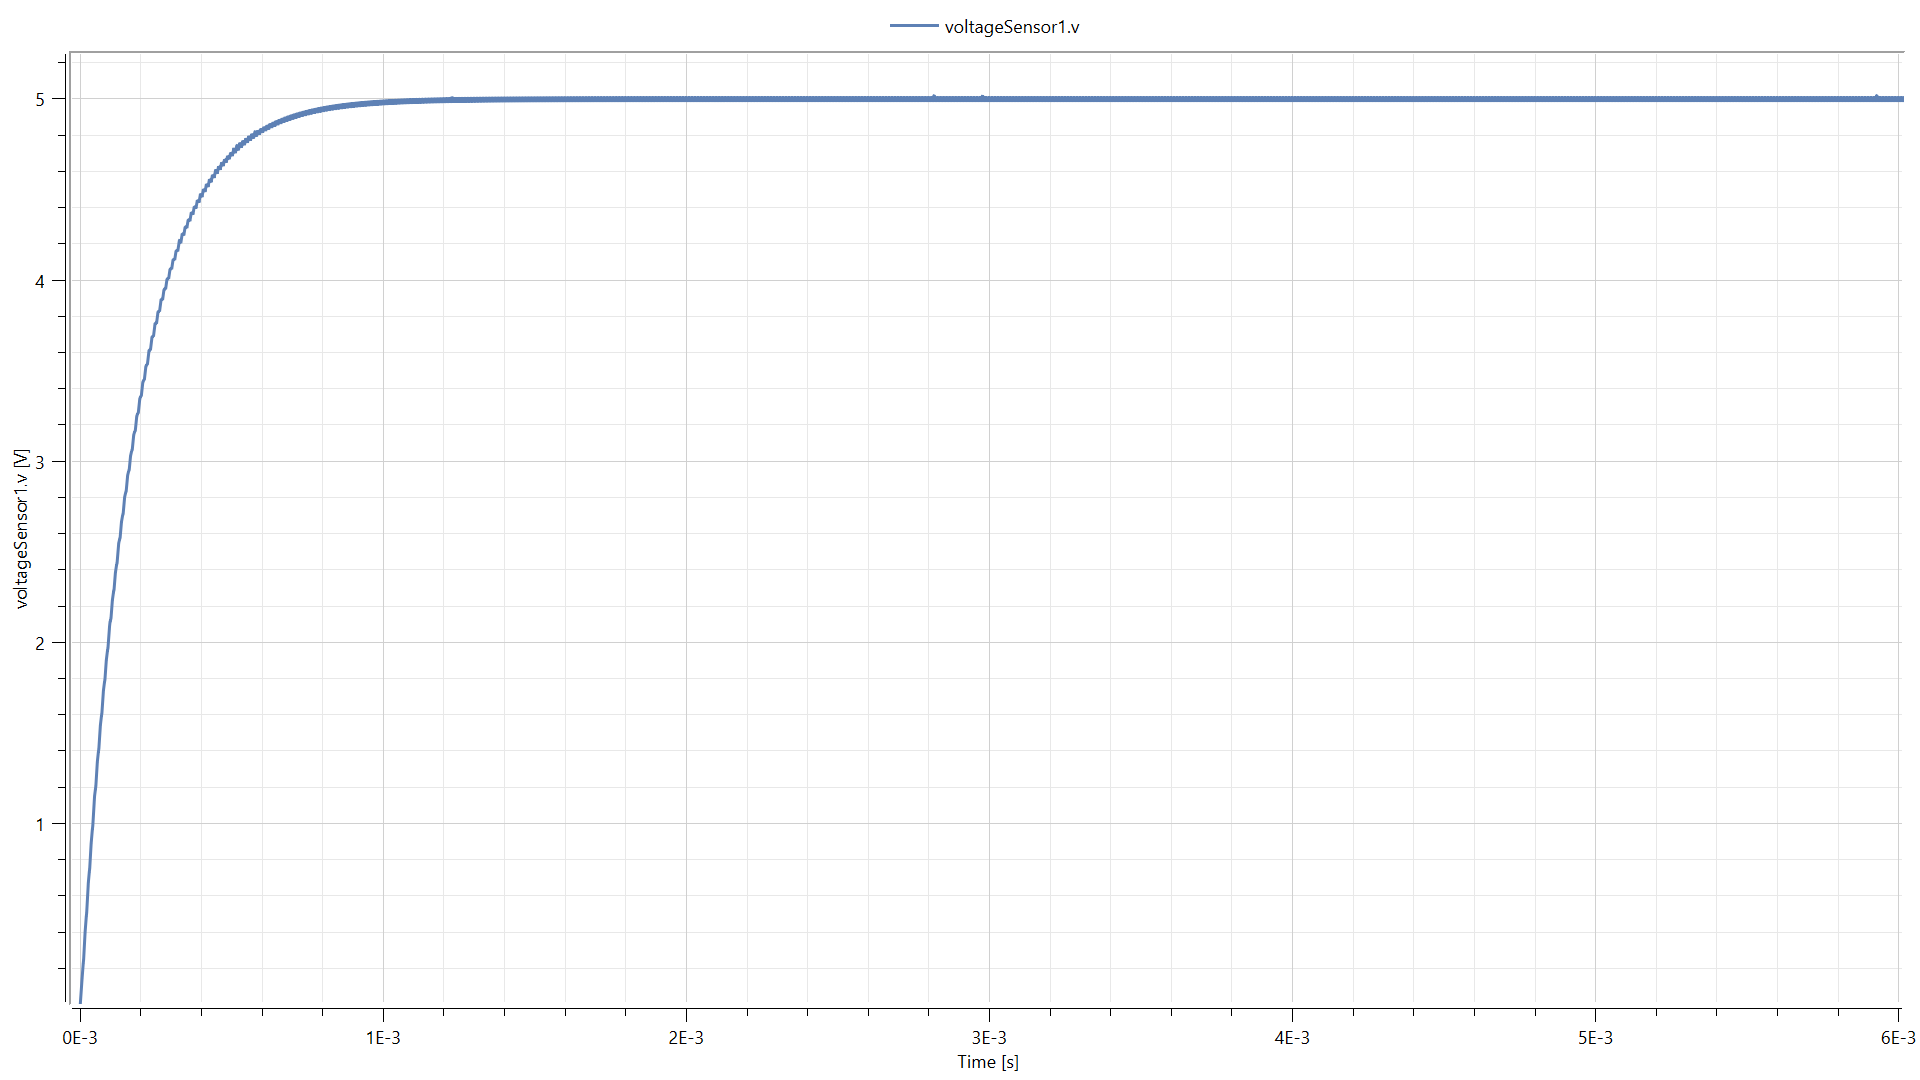
\includegraphics[width=0.6\textwidth]{buck_NI_output_newD}
%     \caption{Non-ideal Buck converter output voltage for duty cycle of 61.44\% and a load of $3.9$ $\Omega$. An average voltage of 5.00 V is observed.}
%     \label{fig:buck_NI_output_newD}
% \end{figure}
\color{red}MISSING GRAPHICS
\color{black}

\newpage
\section{Flyback Converter}
\subsection{Ideal Calculations}
\begin{figure}[htp]
    \centering
    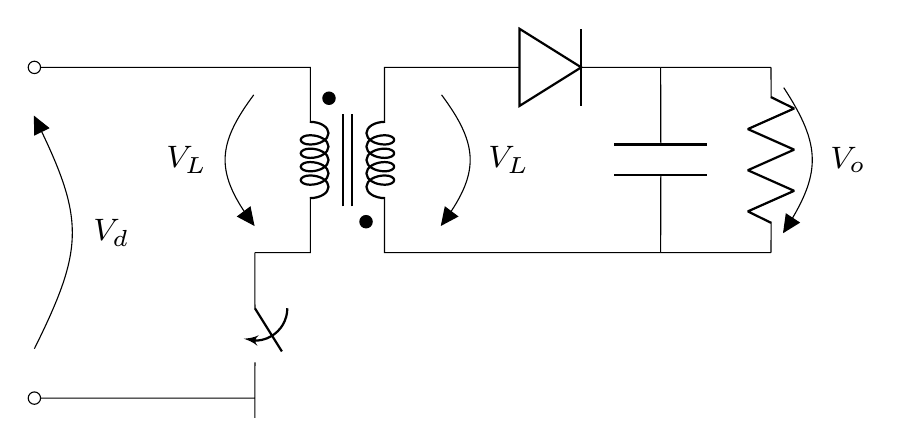
\begin{tikzpicture}[scale=1.4, transform shape]
        % \caption{Ideal Flyback Converter}
        %draw tri and quadpoles
        \node[transformer core, anchor = A1, scale = 0.8](transformer) at (2,2){};
        \node[circ](c1) at (transformer.inner dot A1){};
        \node[circ](c2) at (transformer.inner dot B2){};
        % \node[switch, scale = 0.8](switch1) at (2,0){};
        
        %Primary
        \draw (0,-1)
         to [open,v>=\footnotesize $V_d$,o-o] ++(0,3)
         to (0,2)
         to (2,2)
         to (transformer.A1) % current here
         (transformer.A2) to [switch,transform shape] ++(0,-1.5)
         |- (0,-1);
         
        
        %Secondary
         \draw (transformer.B1) to[Do] ++ (2,0) coordinate(A)
         (A) to[C] (A |- transformer.B2)
         (transformer.B2) to (A |- transformer.B2);
        
         \draw (A) ++(1,0) coordinate(B)
         (A)--(B)
         (B) to [R,v^=\footnotesize $V_o$] (B|- transformer.B2)
         (B|- transformer.B2) -- (A |- transformer.B2);
        
        % \draw (npn.C) to[open shifted, v^=$v_Q$](npn.E);
        % \draw (npn.B) to[open shifted, v=$v_{be}$, voltage shift=-1](npn.E);
        \draw (transformer.A1) to[open shifted, v=\footnotesize $V_L$](transformer.A2);
        \draw (transformer.B1) to[open shifted, v^>=\footnotesize$V_L$](transformer.B2);
        
        
        \end{tikzpicture}
        \label{tikzpicture:idealFlyback}
        \caption{Ideal Flyback Converter}
    \end{figure}
    \noindent
    To determine the required duty cycle for the ideal flyback converter the zero volt seconds rule is applied. 
    It is assumed that no lossed occur at the transformer, switches and diodes. It also assumed that the transform turns ratio is 1:1.
    For the case in which the switch is closed, 
    \begin{equation}
        V_d - V_L = 0
    \end{equation}
    The secondary side has no influence, as the inductor is assumed to be in steady state. 
    For the case where the switch is open,
    \begin{equation}
        -V_L - V_o = 0
    \end{equation}
    The application of the zero-volts second rule,
    \begin{equation}
        DT_s \cdot V_{L \: on} + (1-D)T_s \cdot V_{L\:off} = 0
        \label{equation:zerovoltseconds}
    \end{equation}
    Cancel out $T_s$, then substitute equations $V_L$ equations,
    \begin{equation}
        D \cdot V_d+ (1-D) \cdot -V_o = 0
    \end{equation}
    Therefore, the duty cycle becomes,
    \begin{equation}
        D  = \dfrac{V_o}{V_d+V_o}
    \end{equation}
    The design specifications desire $V_o$ to be 10V but specifys the input, $V_d$, to be a range of [5,12]V
    For $V_{d\:min}$, the duty cycle ends up being,
    \begin{equation}
        D = \dfrac{10}{5+10} = 66.67\:\%
    \end{equation}
    and for $V_{d\:max}$,
    \begin{equation}
        D = \dfrac{10}{12+10} = 45.45\:\%
    \end{equation}
\newpage
\subsection{Ideal Simulations}
\begin{figure}[htp]
    \centering
    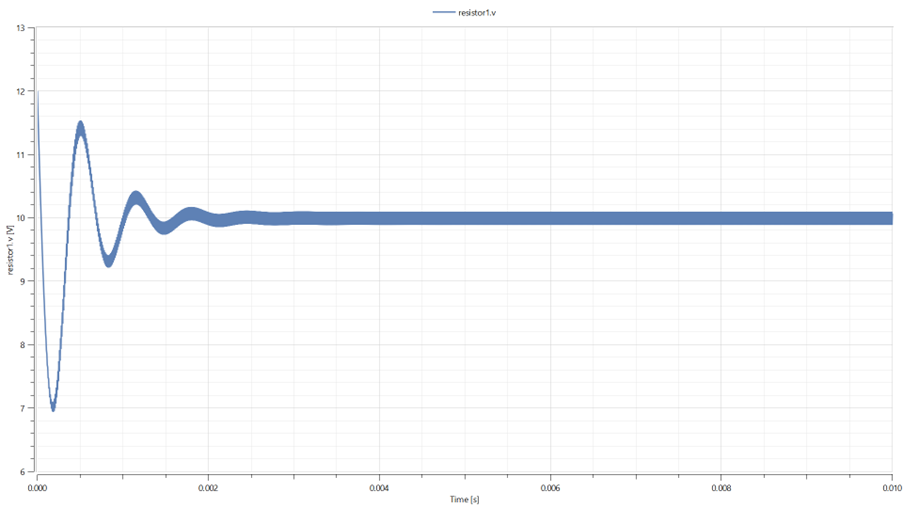
\includegraphics[width=0.75\textwidth]{IdealSim12V.png}
    \caption{Ideal Flyback, Output Voltage $V_o$ = 10 V, ($V_d$ = 12 V, $D$ = 0.4545)}
    \label{fig:IdealSim12V}
\end{figure}

\begin{figure}[htp]
    \centering
    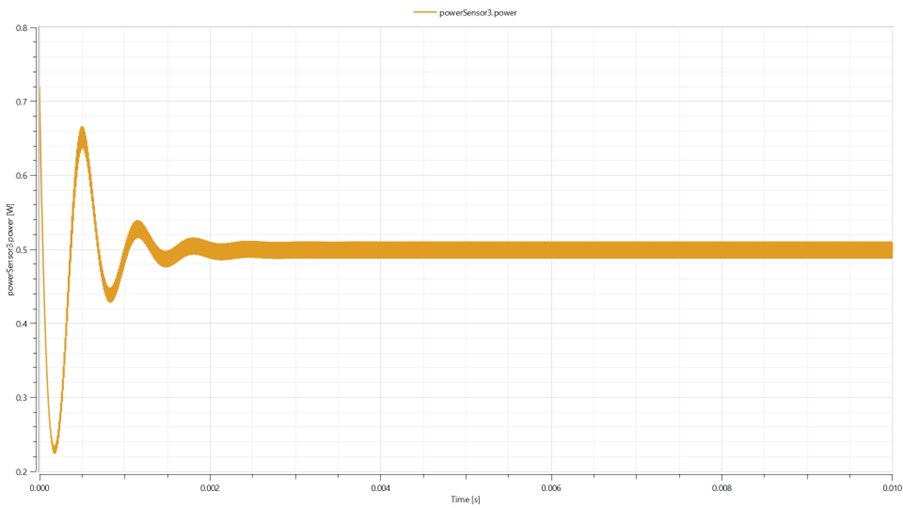
\includegraphics[width=0.75\textwidth]{PowerIdealSim12V.png}
    \caption{Ideal Flyback, Output Power $P_o$ = 0.45 W, ($V_d$ = 12 V, $D$ = 0.4545)}
    \label{fig:PowerIdealSim12V}
\end{figure}

\begin{figure}[htp]
    \centering
    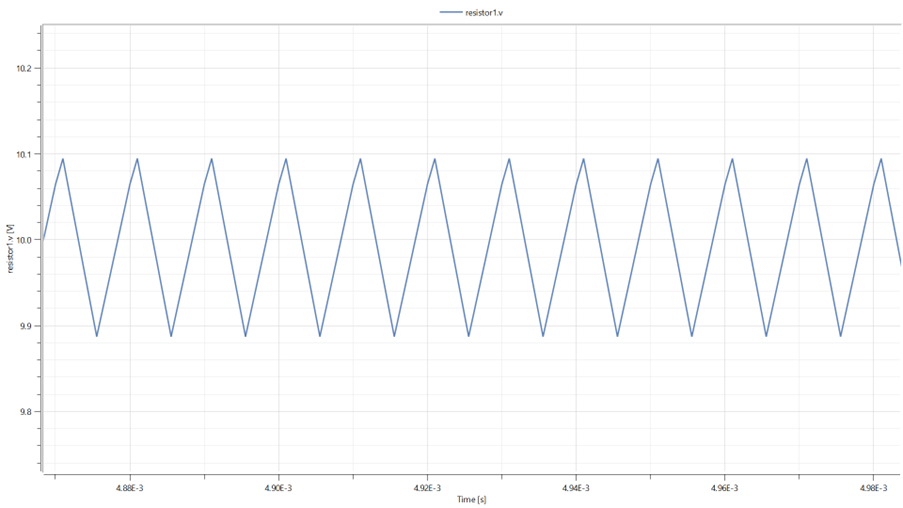
\includegraphics[width=0.75\textwidth]{RippleIdealSim12V.png}
    \caption{Ideal Flyback, Output Ripple $\Delta V_o$ = 0.2 V, ($V_d$ = 12 V, $D$ = 0.4545)}
    \label{fig:RippleIdealSim12V}
\end{figure}
% All simulations met expectations. 
\begin{figure}[htp]
    \centering
    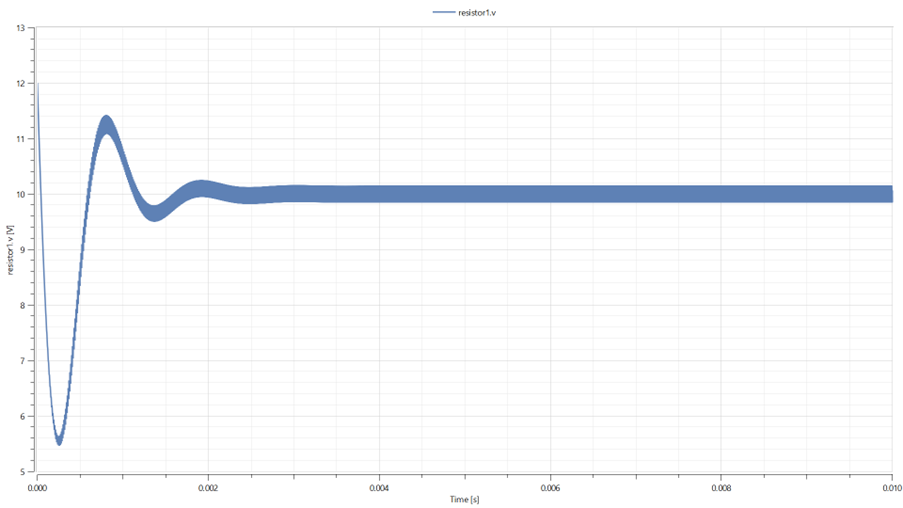
\includegraphics[width=0.75\textwidth]{IdealSim5V.png}
    \caption{Ideal Flyback, Output Voltage $V_o$ = 10 V, ($V_d$ = 5 V, $D$ = 0.6667)}
    \label{fig:IdealSim5V}
\end{figure}

\begin{figure}[htp]
    \centering
    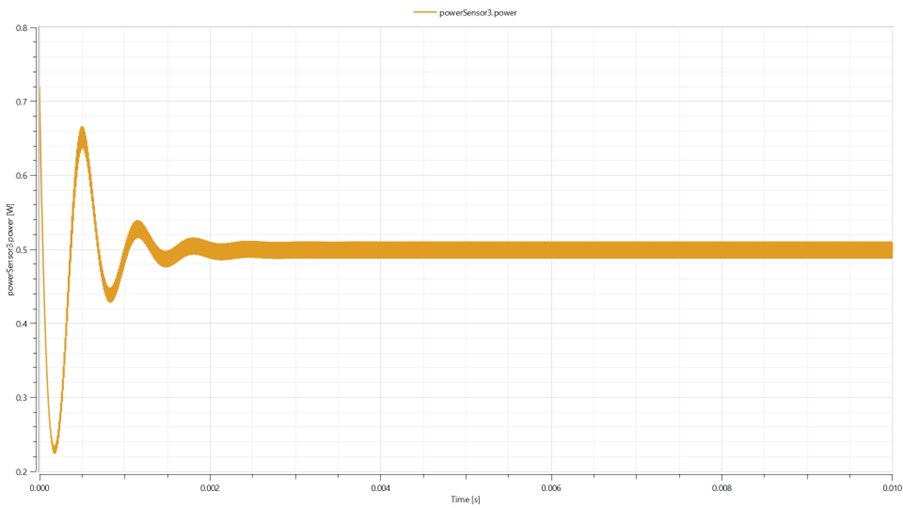
\includegraphics[width=0.75\textwidth]{PowerIdealSim12V.png}
    \caption{Ideal Flyback, Output Power $P_o$ = 0.45 W, ($V_d$ = 5 V, $D$ = 0.6667)}
    \label{fig:PowerIdealSim5V}
\end{figure}

\begin{figure}[htp]
    \centering
    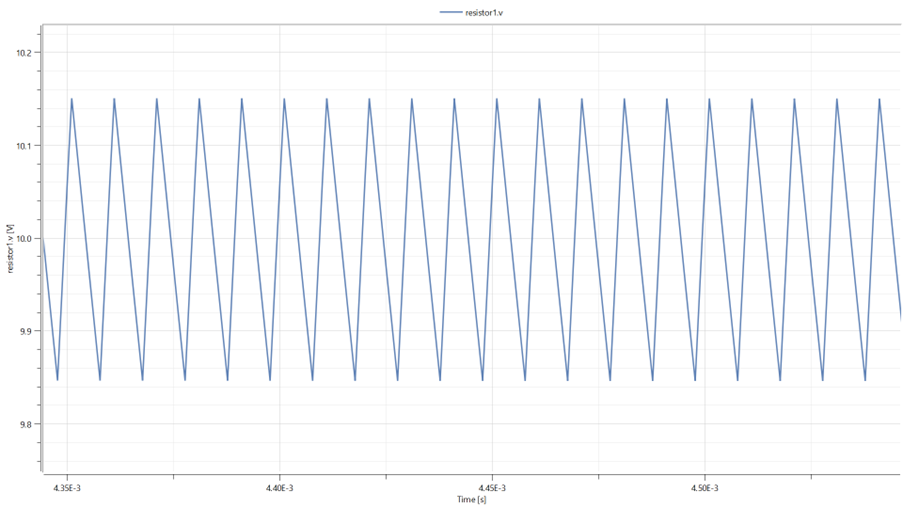
\includegraphics[width=0.75\textwidth]{RippleIdealSim5V.png}
    \caption{Ideal Flyback, Output Ripple $\Delta V_o$ = 0.3V, ($V_d$ = 5 V, $D$ = 0.6667)}
    \label{fig:RippleIdealSim5V}
\end{figure}


\newpage
\subsection{Non-Ideal Calculations}
\begin{figure}[htp]
    \centering
    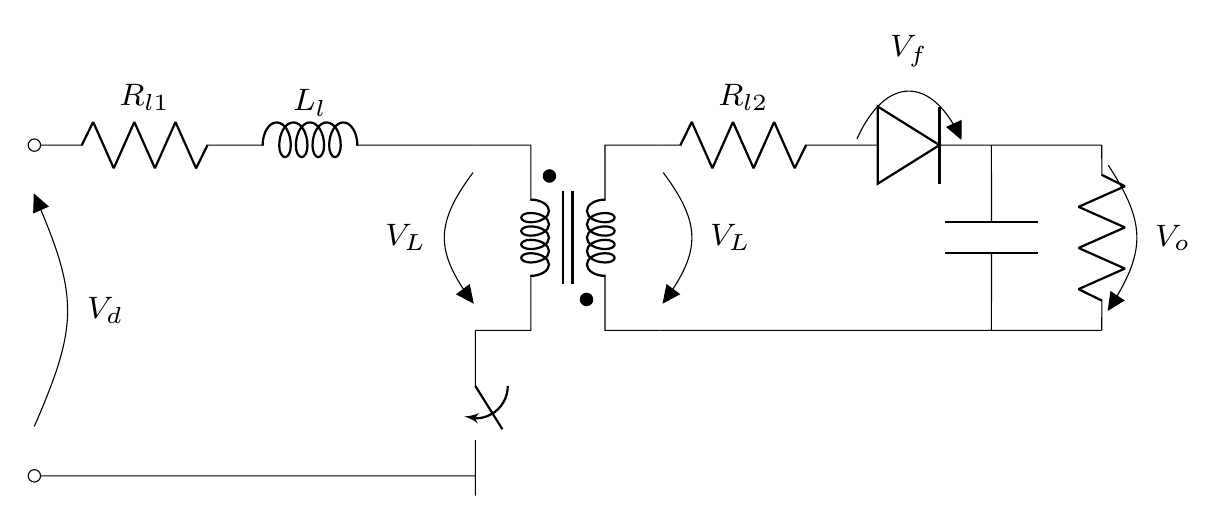
\begin{tikzpicture}[scale=1.4, transform shape,voltage shift=-0.5]
        % \caption{Ideal Flyback Converter}
        %draw tri and quadpoles
        \node[transformer core, anchor = A1, scale = 0.8](transformer) at (2,2){};
        \node[circ](c1) at (transformer.inner dot A1){};
        \node[circ](c2) at (transformer.inner dot B2){};
        % \node[switch, scale = 0.8](switch1) at (2,0){};
        
        %Primary
        \draw (-2,-1)
         to [open,v>=\footnotesize $V_d$,o-o] ++(0,3)
         to (-2,2)
         to [R,l^=\footnotesize $R_{l1}$,label distance = 2pt] (0,2)
         to [L,l^=\footnotesize $L_{l}$] (1,2)
         to (transformer.A1) % current here
         (transformer.A2) to [switch,transform shape] ++(0,-1.5)
         |- (-2,-1);
         
        
        %Secondary
         \draw (transformer.B1)
        %  to [L,l^=\footnotesize $L_{l2}$] ++(1.5,0)
         to [R,l^=\footnotesize $R_{l2}$,label distance = 2pt] ++(1.5,0)
         to [Do,v^=\footnotesize $V_f$] ++(1.5,0) coordinate(A)
         (A) to [C] (A |- transformer.B2)
         (transformer.B2) to (A |- transformer.B2);
        
         \draw (A) ++(1,0) coordinate(B)
         (A)--(B)
         (B) to [R,v^=\footnotesize $V_o$] (B|- transformer.B2)
         (B|- transformer.B2) -- (A |- transformer.B2);
        
        % \draw (npn.C) to[open shifted, v^=$v_Q$](npn.E);
        % \draw (npn.B) to[open shifted, v=$v_{be}$, voltage shift=-1](npn.E);
        \draw (transformer.A1) to[open shifted, v=\footnotesize $V_L$,voltage shift=-0.8](transformer.A2);
        \draw (transformer.B1) to[open shifted, v^>=\footnotesize$V_L$,voltage shift=-0.8](transformer.B2);
        
        
        \end{tikzpicture}
        \label{tikzpicture:nonidealFlyback}
        \caption{Non-Ideal Flyback Converter}
    \end{figure}
    \noindent The specifications for the flyback converter ask for an output of 10 V at 0.5 W. 
    To achieve this, an average current can be calculated using ohm's law of power,
    \begin{equation}
        P = IV
    \end{equation}
    which gives $I_{avg}$ = 50 mA. This can be used to determine the load resistance with ohm's law,
    \begin{equation}
        V = IR
    \end{equation}
    Therefore, the load resistance, $R_L$ is $200\: \Omega$. The closest available load resistor is $220\: \Omega$ which can be reversed to get the average current,
    $I_{avg}$ = 45.45 mA and output power, $P = 0.4545$ W which will be used for further calculations.
    The non-ideal components of the current flyback converter can be 
    modelled like this. The primary side is the only active when the 
    switch is on, this means the internal MOSFET resistance and the internal 
    transformer resistance can be added together like this,
    \begin{equation}
        R_{l1} = R_{mosfet} + R_{transformer}
        \label{equation:Rp}
    \end{equation}
    For the case when switch is closed,
    \begin{equation}
        V_d - V_{Rl1} - V_{Ll} - V_L = 0
    \end{equation}
    The voltage across the leakage inductance cannot be known, instead the 
    leakage inductance will be ratioed in terms of the magnetising inductance. The magnetising 
    inductance is $3$ mH and the leakage inductance at the primary side is $9\:\mu$H. Therefore the case when
    the switch is closed is simplified to,
    \begin{equation}
        V_d - V_{Rl1} - V_L = 0
    \end{equation}
    Therefore the case for the switch is open,
    \begin{equation}
        -\dfrac{3}{3.009}V_L - V_{Rl2} - V_f - V_o = 0
    \end{equation}
    Applying the zero volt seconds rule, \ref{equation:zerovoltseconds}, and cancelling out Ts,
    \begin{equation}
        D \cdot( V_d - V_{Rl1} ) + (1-D) \cdot \dfrac{3.009}{3}(- V_{Rl2} - V_f - V_o) = 0
    \end{equation}
    rearranging to make duty cycle the subject,
    \begin{equation}
        D  = \frac{\dfrac{3.009}{3}(V_{Rl2} + V_f + V_o)}{V_d - V_{Rl1} + \dfrac{3.009}{3}(V_{Rl2} + V_f + V_o)}
    \end{equation}
    Equation \ref{equation:Rp}, is used to calculate $R_{l1} = 1.47$ and referring to the 
    calculated average current, $I_{avg} = 45.45$ mA. The duty cycle can 
    be calculated for the maximum and minimum of the desired $V_d$ range [5,12]V. For $V_{d\:max}$,
    \begin{equation}
        D  = \frac{\dfrac{3.009}{3}(1.7\cdot I_{avg} + 0.7 + 10)}{12 - 1.47\cdot I_{avg} + \dfrac{3.009}{3}(1.7\cdot I_{avg} + 0.7 + 10)} = 47.53\: \%
    \end{equation}
    and for $V_d\:min$,
    \begin{equation}
        D  = \frac{\dfrac{3.009}{3}(1.7\cdot I_{avg} + 0.7 + 10)}{5 - 1.47\cdot I_{avg} + \dfrac{3.009}{3}(1.7\cdot I_{avg} + 0.7 + 10)} = 68.66\: \%
    \end{equation}

\newpage

\subsection{Non-Ideal Simulations}
\begin{figure}[htp]
    \centering
    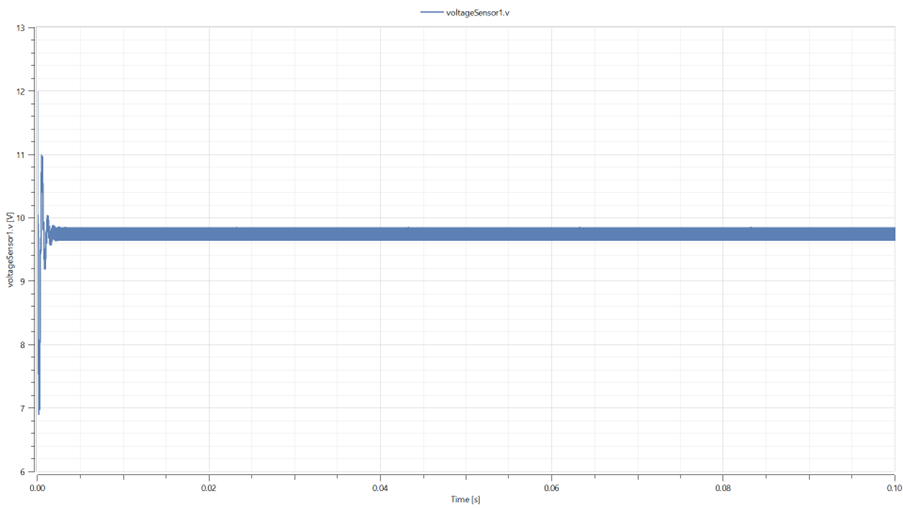
\includegraphics[width=0.75\textwidth]{NonIdealSim12V(calculated).png}
    \caption{Non Ideal Flyback, Output Voltage $V_o$ = 9.746 V, ($V_d$ = 12 V, $D$ = 0.4753)}
    \label{fig:NonIdealSim12Vcal}
\end{figure}

\begin{figure}[htp]
    \centering
    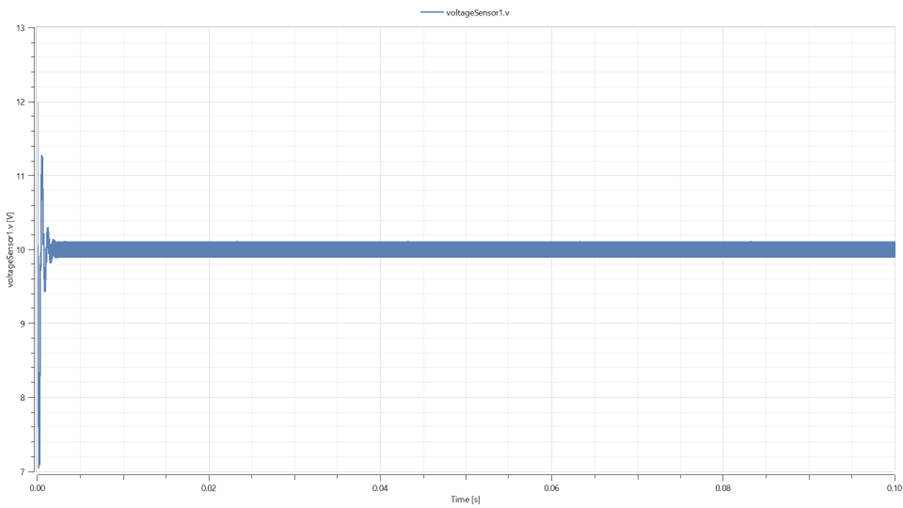
\includegraphics[width=0.75\textwidth]{NonIdealSim12V(tested).png}
    \caption{Non Ideal Flyback, Output Voltage $V_o$ = 10 V, ($V_d$ = 12 V, $D$ = 0.4815)}
    \label{fig:NonIdealSim12Vtested}
\end{figure}

\begin{figure}[htp]
    \centering
    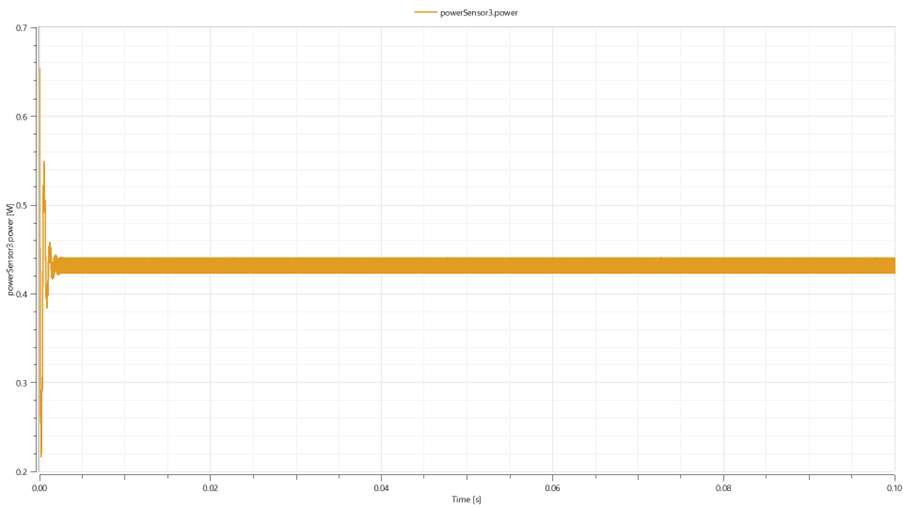
\includegraphics[width=0.75\textwidth]{PowerNonIdealSim12V.png}
    \caption{Non Ideal Flyback, Output Power $P_o$ = 0.432 W, ($V_d$ = 12 V, $D$ = 0.4753)}
    \label{fig:PowerNonIdealSim12V}
\end{figure}

\begin{figure}[htp]
    \centering
    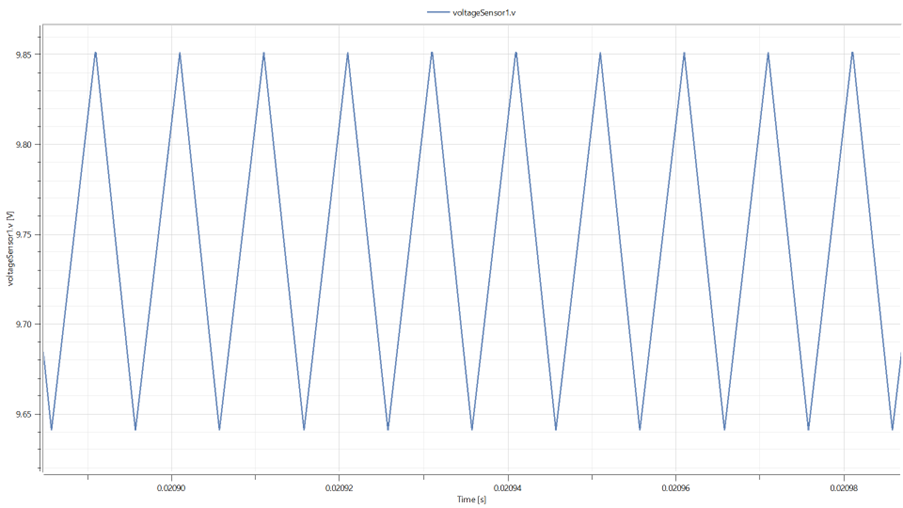
\includegraphics[width=0.75\textwidth]{RippleNonIdealSim12V.png}
    \caption{Non Ideal Flyback, Output Ripple $\Delta V_o$ = 210 mV, ($V_d$ = 12 V, $D$ = 0.4753)}
    \label{fig:RippleNonIdealSim12V}
\end{figure}
% All simulations met expectations. 
\begin{figure}[htp]
    \centering
    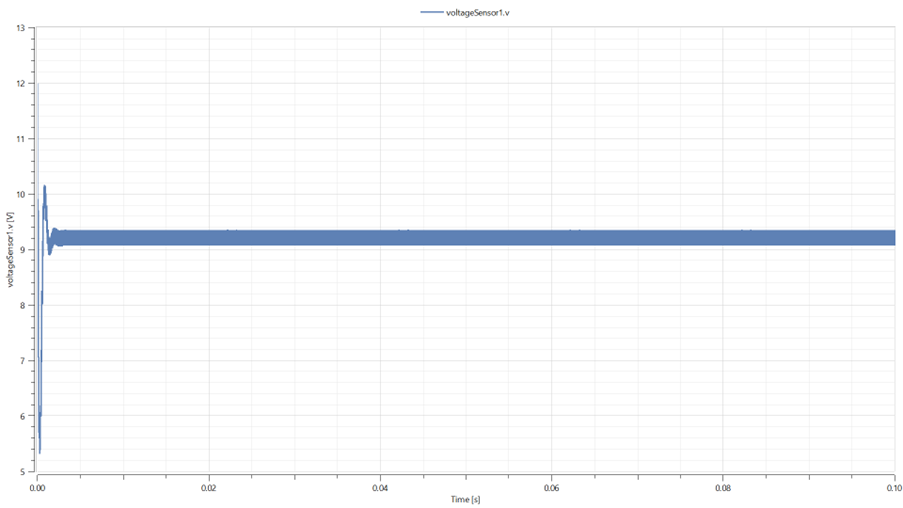
\includegraphics[width=0.75\textwidth]{NonIdealSim5V(calculated).png}
    \caption{Non Ideal Flyback, Output Voltage $V_o$ = 9.21 V, ($V_d$ = 5 V, $D$ = 0.6866)}
    \label{fig:NonIdealSim5Vcal}
\end{figure}

\begin{figure}[htp]
    \centering
    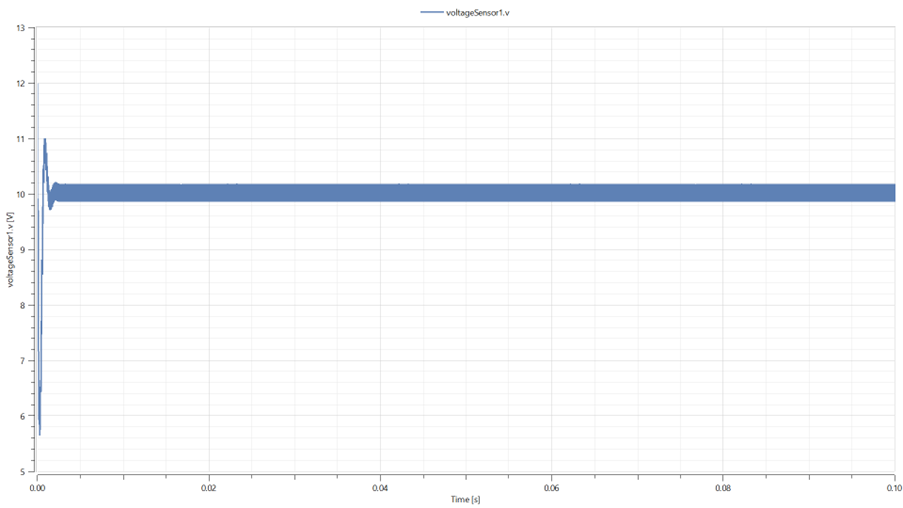
\includegraphics[width=0.75\textwidth]{NonIdealSim5V(tested).png}
    \caption{Non Ideal Flyback, Output Voltage $V_o$ = 10.02 V, ($V_d$ = 5 V, $D$ = 0.7055)}
    \label{fig:NonIdealSim5Vtested}
\end{figure}

\begin{figure}[htp]
    \centering
    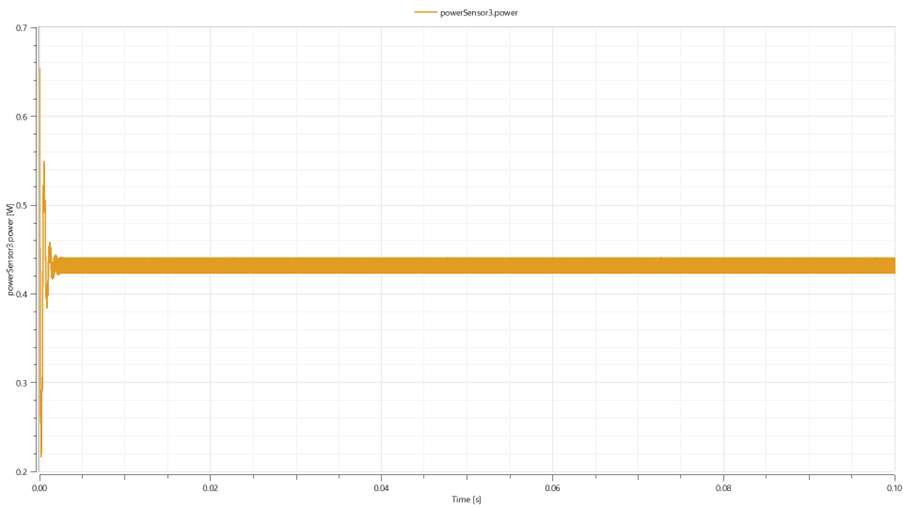
\includegraphics[width=0.75\textwidth]{PowerNonIdealSim12V.png}
    \caption{Non Ideal Flyback, Output Power $P_o$ = 0.385 W, ($V_d$ = 5 V, $D$ = 0.6667)}
    \label{fig:PowerNonIdealSim5V}
\end{figure}

\begin{figure}[htp]
    \centering
    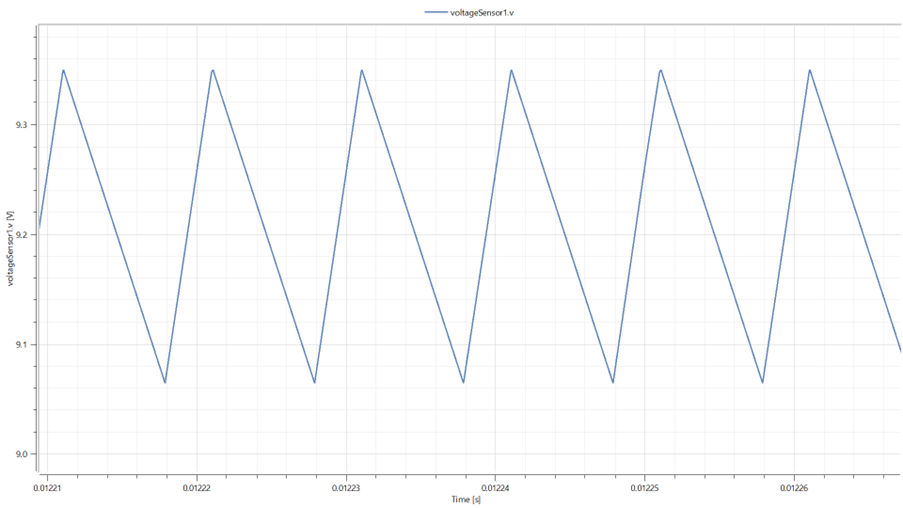
\includegraphics[width=0.75\textwidth]{RippleNonIdealSim5V.png}
    \caption{Non Ideal Flyback, Output Ripple $\Delta V_o$ = 290 mV, ($V_d$ = 5 V, $D$ = 0.6667)}
    \label{fig:RippleNonIdealSim5V}
\end{figure}
\newpage
\subsection{Results}

\begin{figure}[htp]
    \centering
    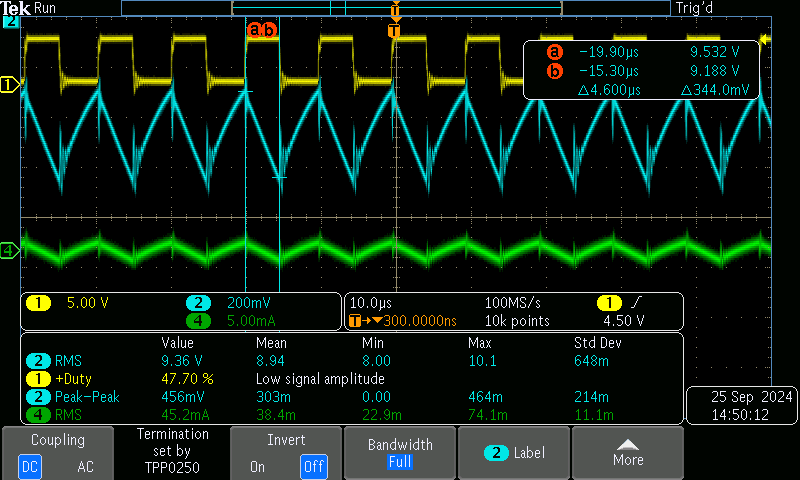
\includegraphics[width=0.7\textwidth]{Flyback/tek0001.png}
    \caption{Practical Flyback, Ripple $\Delta V_o$ = 344 mV, ($C$ = 1 $\mu$F, $V_d$ = 12 V, $D$ = 0.477)}
    \label{fig:Practical1}
\end{figure}

\begin{figure}[htp]
    \centering
    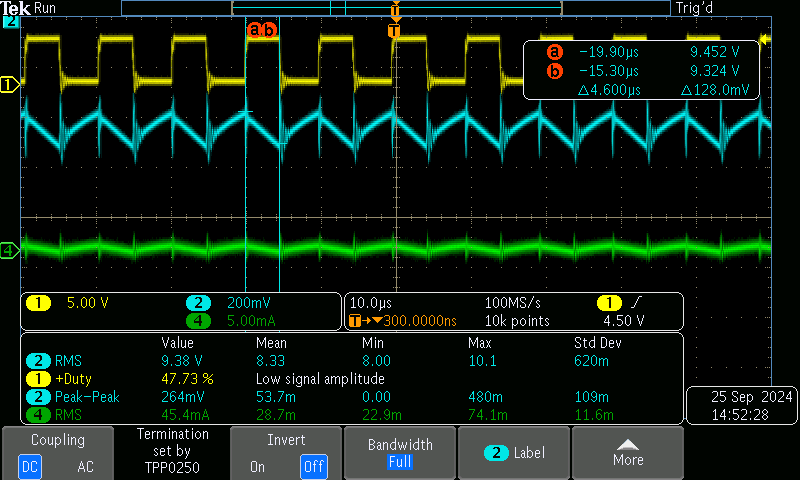
\includegraphics[width=0.7\textwidth]{Flyback/tek0002.png}
    \caption{Practical Flyback, Ripple $\Delta V_o$ = 128 mV, ($C$ = 2.68 $\mu$F, $V_d$ = 12 V, $D$ = 0.477)}
    \label{fig:Practical2}
\end{figure}

\begin{figure}[htp]
    \centering
    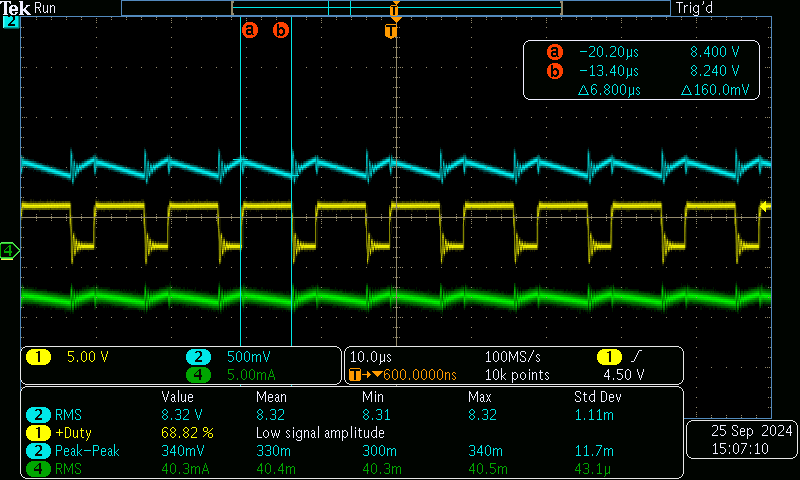
\includegraphics[width=0.7\textwidth]{Flyback/tek0003.png}
    \caption{Practical Flyback, Output Voltage $V_o$ = 8.32 V, ($C$ = 2.68 $\mu$F, $V_d$ = 5 V, $D$ = 0.688)}
    \label{fig:Practical3}
\end{figure}

\begin{figure}[htp]
    \centering
    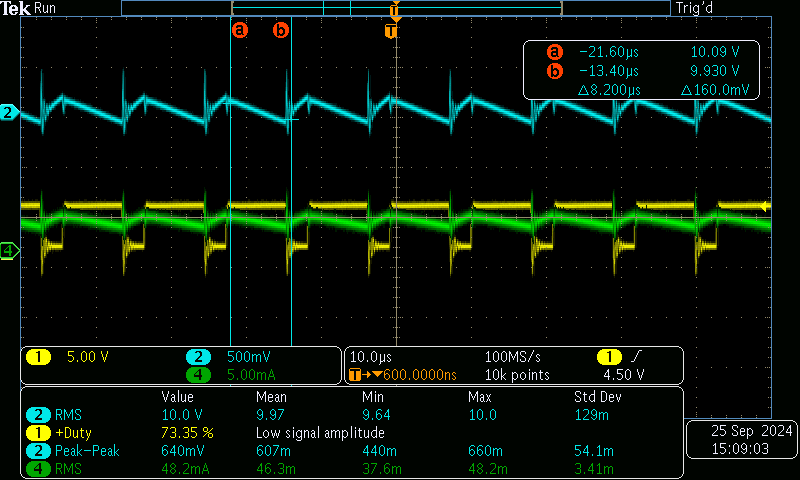
\includegraphics[width=0.7\textwidth]{Flyback/tek0004.png}
    \caption{Practical Flyback, Output Voltage $V_o$ = 10 V, ($C$ = 2.68 $\mu$F, $V_d$ = 5 V, $D$ = 0.734)}
    \label{fig:Practical4}
\end{figure}
\newpage
\subsection{Conclusion}

\newpage
\bibliographystyle{IEEEtranN}
\bibliography{references}

\end{document}
